% CAPÍTULO HISTÓRICO
% juntamente com cronologia e genealogia

% Que problema motivou sua criação?
% Como a linguagem evoluiu em sintaxe, semântica e implementação?
% Como a comunidade e as instituições influenciaram seu desenvolvimento?
% Que aplicações impulsionaram seu uso?
% Qual é o estado atual e o legado de Prolog?

% Quando e onde a linguagem surgiu?
Prolog teve sua versão preliminar criada no final de 1971, e uma versão mais
definitiva no final de 1972, na Université Grenoble Alpes, onde em fevereiro
deste mesmo ano, conseguiram um investimento de 122.000,00 Francos Franceses,
que valem o equivalente a R\$ 802.055,43 (consultado em 18/09/2026),
distribuídos em um período de 18 meses, vindo de investimentos de uma
instituição afiliada ao Ministério da Indústria da França. 

Com este investimento, compraram um terminal teletipo de 30 caracteres por
segundo, conectado ao IBM 360-67, um computador que para os padrões da época,
era muito bom, podendo chegar até 4 \emph{megabytes} de memória na sua
configuração intermediária. Em Birth of Prolog, descreveram esta máquina como
``a mais conveniente disponível''. 
% citar de onde veio a conversão francos para euros para BRL:
% https://inflationhistory.com/en-US/?currency=FRF&amount=122000&year=1972

\begin{figure}[htb]
   \caption{IBM S/360 Model 67}

   \begin{center}
       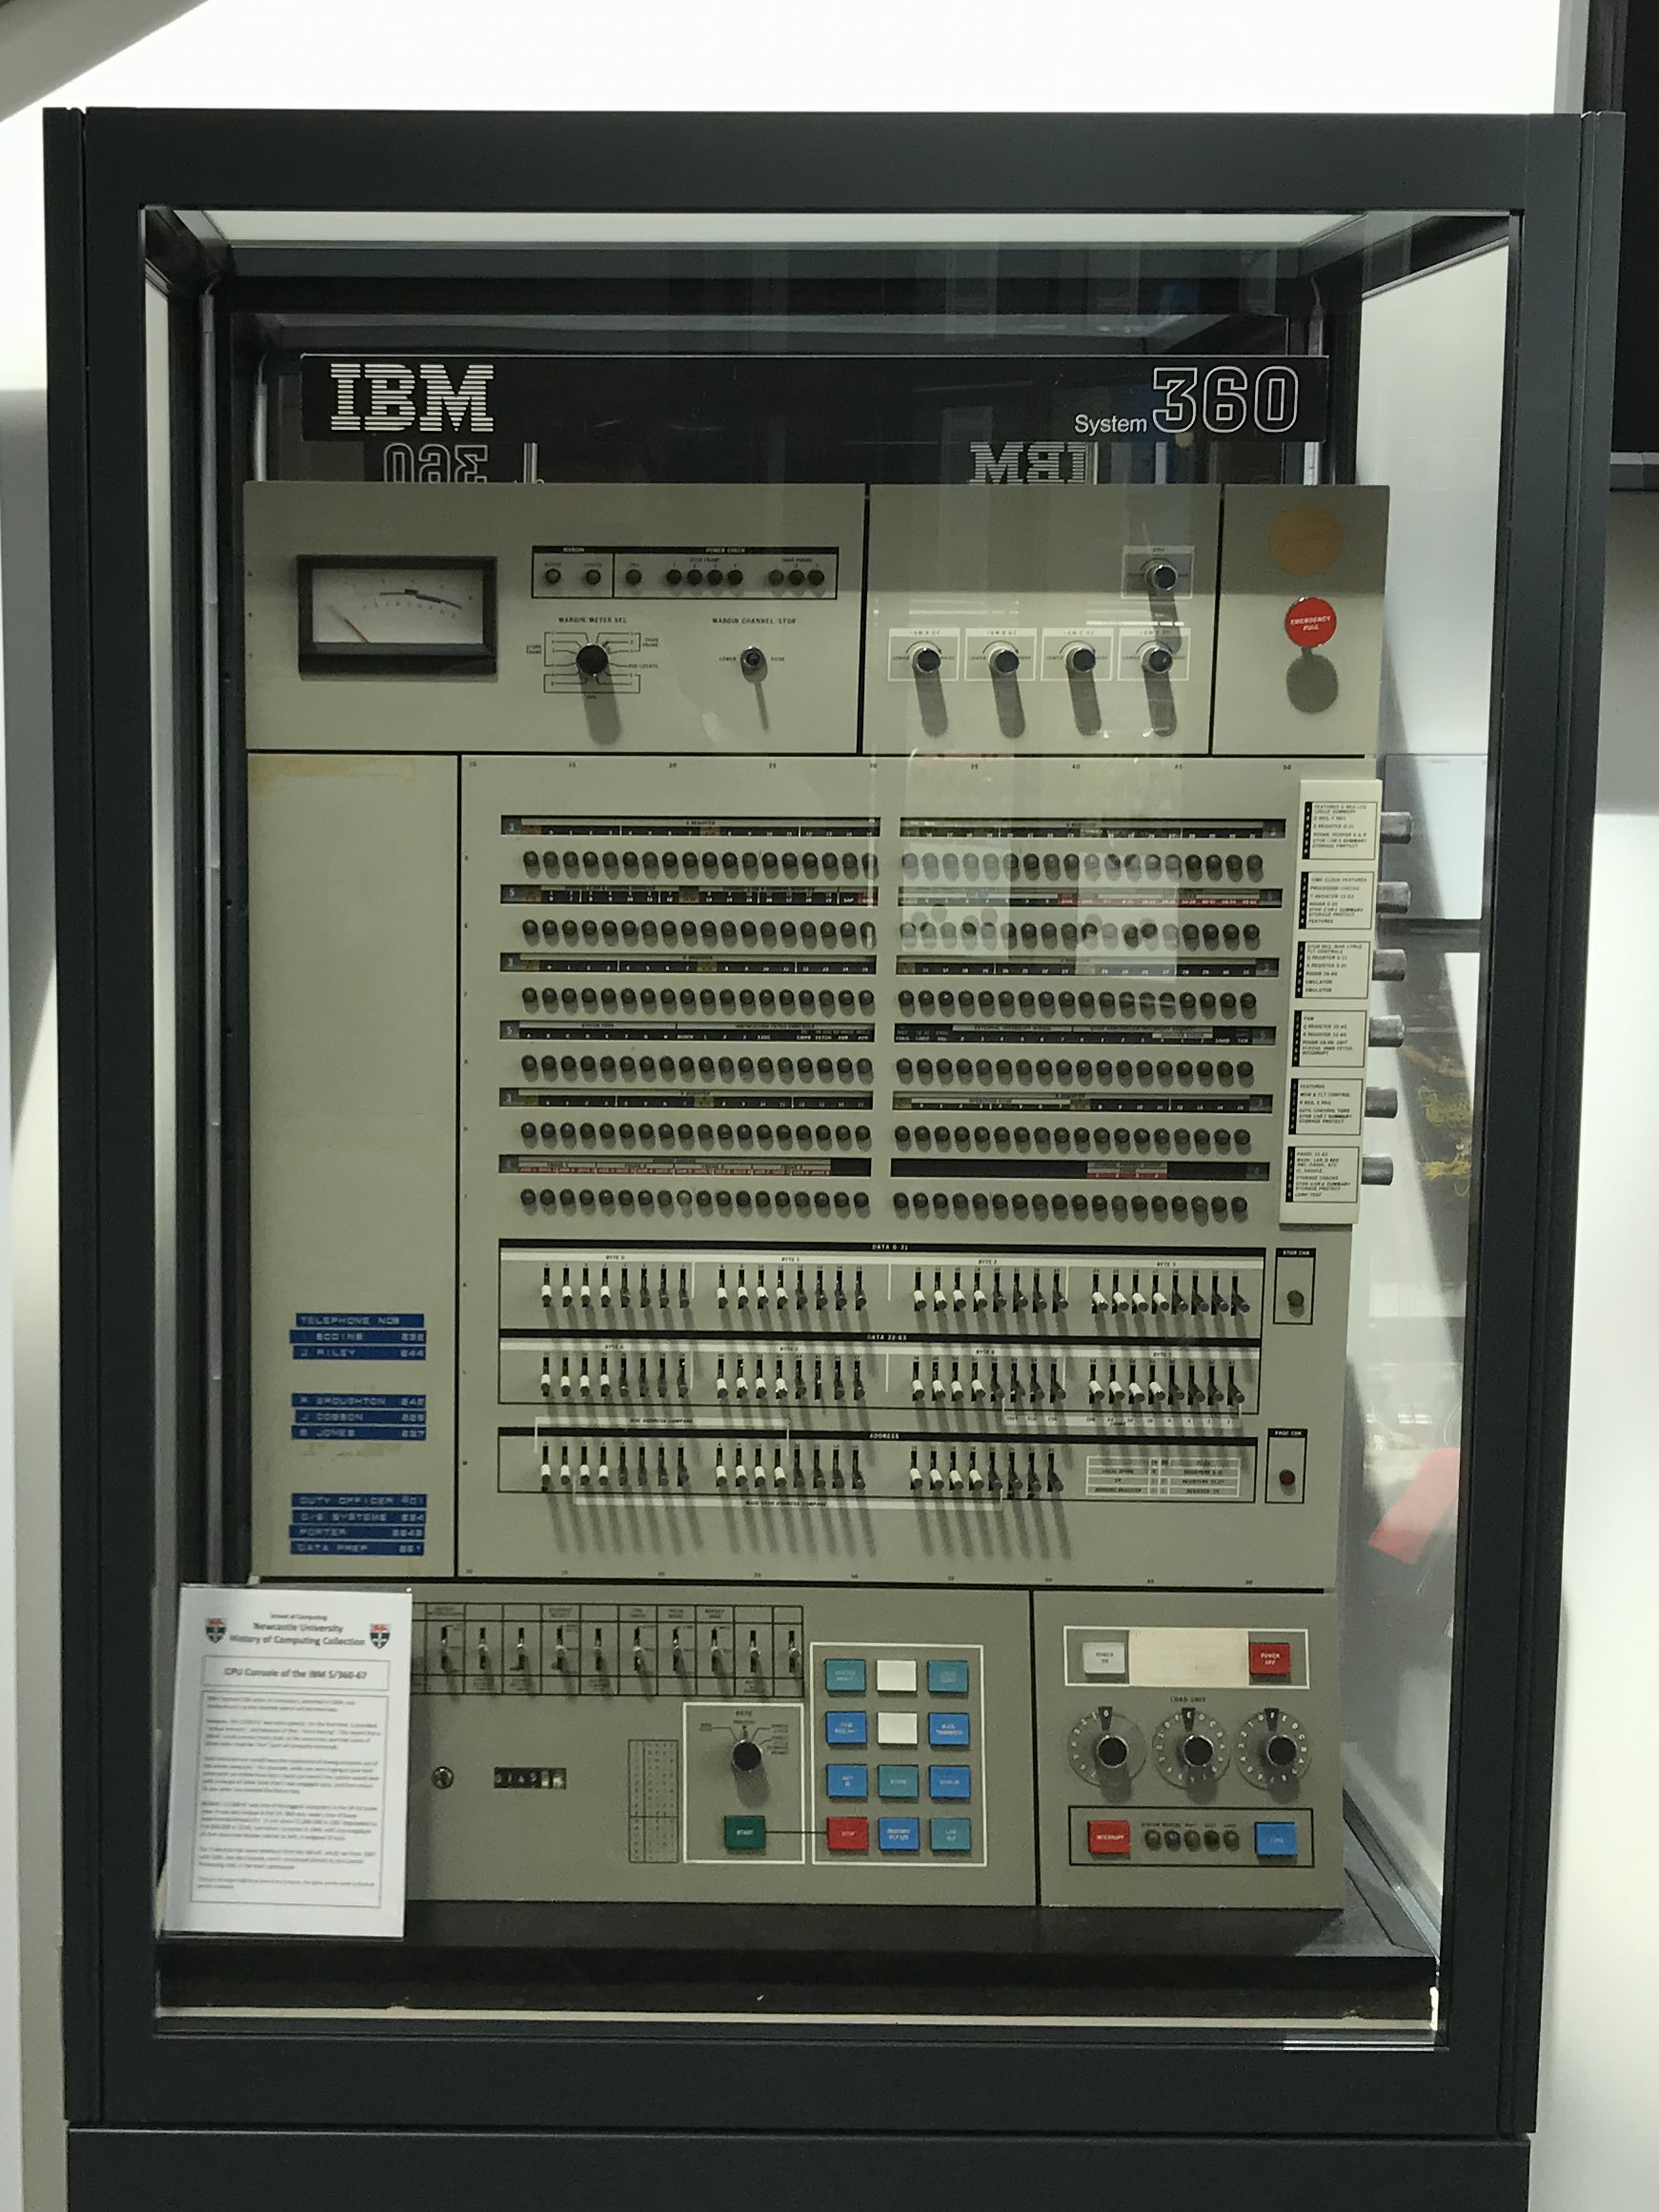
\includegraphics[width=0.6\textwidth]{figuras/IBM360_67.jpg}
   \end{center}

   \legend{Fonte: \cite{ncl_cs_history_ibm360}, Adaptado}
\end{figure}

\chapter{Quem foram seus criadores e colaboradores}
Robert Pasero
Philippe Rousseel
Alain Colmerauer
Jean Trudel
Robert Kowalski
Henry Kanoui
Maarten van Emden
Niklaus Wirt
Roger Boyer
Jay Moore
Gérard Battani
Henry Méloni
René Bazzoli
David Warren

% Quais versões, padrões e implementações marcaram época? talvez "marcante" para
% um título de capítulo não seja muito apropriado, bom pensar ou em um título
% alternativo, ou outra palavra
\chapter{Versões, padrões e implementações marcantes}
\begin{figure}[htb]
    \caption{Timeline aproximada de alguns sistemas em Prolog (até o padrão ISO).}

    \begin{center}
        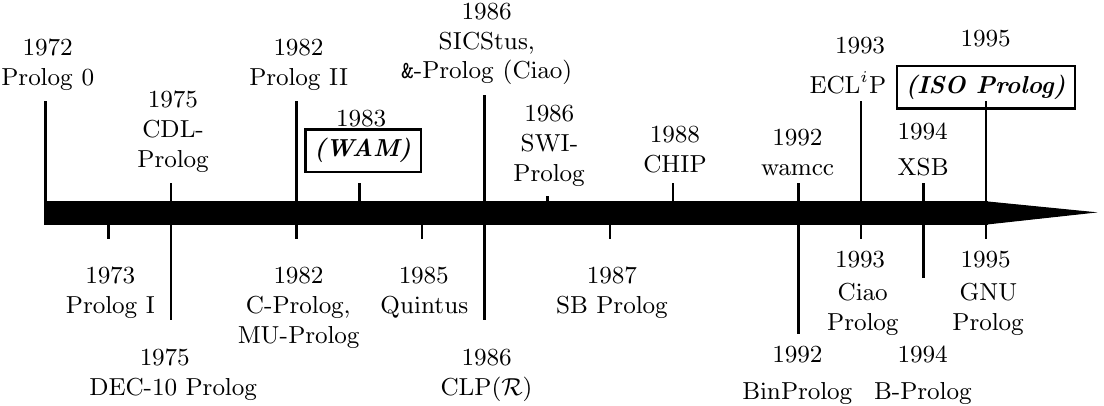
\includegraphics[width=1\textwidth]{figuras/timeline.png}
    \end{center}

    \legend{Fonte: \cite{korner2022fiftyyearsprolog}. Adaptado}
\end{figure}

% \begin{verbatim}
%     Usuário:    Gatos matam ratos.
%                 Tom é um gato que não gosta de ratos que comem queijo.
%                 Jerry é um rato que come queijo.
%                 Max não é um rato.
%                 O que o Tom faz?
%     Computador: Tom não gosta de ratos que comem queijo.
%                 Tom mata ratos.
%     Usuário:    Quem é um gato?
%     Computador: Tom.
%     Usuário:    O que Jerry come?
%     Computador: Queijo.
%     Usuário:    Quem não gosta de ratos que comem queijo?
%     Computador: Tom.
%     Usuário:    O que Tom come?
%     Computador: O que gatos que não gostam de ratos que comem queijo comem.
% \end{verbatim}
% \cite{Colmerauer1993-cj}, Adaptado